\documentclass[11pt]{article}
\usepackage[margin=1in]{geometry}
\usepackage{amsmath,amssymb,graphicx,booktabs,xcolor,fancyvrb}
\usepackage[colorlinks=true,linkcolor=blue]{hyperref}

\makeatletter
\def\ps@hw{%
  \def\@oddhead{\itshape\small CS 334 HW2 --- Written Submission\hfill Nathaniel Schrader}%
  \def\@oddfoot{\hfil\small\thepage\hfil}%
  \let\@evenhead\@oddhead \let\@evenfoot\@oddfoot}
\makeatother
\pagestyle{hw}

\fvset{fontsize=\footnotesize,frame=single,numbers=left,numbersep=4pt,xleftmargin=6pt}
\newcommand{\R}{\mathbb{R}}
\newcommand{\vth}{\vec\theta}
\newcommand{\x}[1]{\vec x^{(#1)}}

\begin{document}
\thispagestyle{hw}

\begin{center}
{\Large\bfseries CS 334 --- Homework 2 Submission}\\[4pt]
{\large Nathaniel Schrader \quad|\quad CS 334 Section 2 \quad|\quad Fall 2026}\\[10pt]
\fbox{\parbox{0.92\textwidth}{\small\centering
\textbf{Honor Code Statement:}\\
THIS HOMEWORK IS MY OWN WORK, WRITTEN WITHOUT COPYING FROM OTHER STUDENTS
OR DIRECTLY FROM LARGE LANGUAGE MODELS SUCH AS CHATGPT.\\
Any collaboration or external resources have been properly acknowledged.\\[4pt]
\textit{Nathaniel Schrader}}}
\end{center}
\vspace{6pt}
\hrule
\vspace{10pt}

%=====================================================================
\section*{1\quad Decision Boundaries (24 pts)}

I count a point on the boundary ($\vth\cdot\vec x+b=0$) as misclassified.

\subsection*{(a)}

\paragraph{i. (4pts)} \textbf{No.} With $b=0$, the input $[0,0,0]$ gives $\vth\cdot\vec 0=0$ for any $\vth$, so it's always on the boundary and always wrong.

\paragraph{ii. (4pts)} \textbf{Yes.} $\vth=[1,1,1]^T$, $b=-2.5$. Then $\vth\cdot\vec x+b=x_1+x_2+x_3-2.5$, which is $0.5>0$ for $[1,1,1]$ and at most $-0.5<0$ for every other input.

\subsection*{(b)}

\noindent Positives are $[1,1],[-1,-1]$ and negatives are $[-1,0],[0,1]$.

\paragraph{i. (4pts)} \textbf{Possible.} The positives are distance $\sqrt2$ from the origin and the negatives are distance 1. Use $r=1.2$ with inside = negative and outside = positive.

\paragraph{ii. (4pts)} \textbf{Not possible.} The scores for $[1,1]$ and $[-1,-1]$ are $a+b$ and $-(a+b)$, which always have opposite signs (or are both 0). So both positives can't be on the positive side.

\paragraph{iii. (4pts)} \textbf{Possible.} Center $[-0.5,0.5]$, $s=2$, inside = negative. Inside means $\max(|x_1+0.5|,|x_2-0.5|)<1$. Both negatives give $0.5$ (inside), and both positives give $1.5$ (outside).

\paragraph{iv. (4pts)} \textbf{Possible.} $\alpha=45^\circ$, $s=2$, inside = negative. After rotating, inside means $\max\big(|x_1+x_2|,|x_1-x_2|\big)/\sqrt2<1$. The negatives give $1/\sqrt2\approx0.71$ (inside) and the positives give $2/\sqrt2\approx1.41$ (outside).

%=====================================================================
\section*{2\quad Perceptron Algorithm with Offset (24 pts)}

\paragraph{(a) (4pts)} Each mistake on point $i$ adds $y^{(i)}\x i$ to $\vth$ and $y^{(i)}$ to $b$, and this happens $\alpha_i$ times. Starting from 0:
\[
\vth=\sum_{i=1}^{n}\alpha_i\,y^{(i)}\x i,\qquad b=\sum_{i=1}^{n}\alpha_i\,y^{(i)}
\]

\paragraph{(b) (4pts)} The distance from a point $\vec p$ to the boundary is $\dfrac{\vth\cdot\vec p+b}{\|\vth\|}$: take any $\vec x_0$ on the boundary and project $\vec p-\vec x_0$ onto the unit normal $\vth/\|\vth\|$, using $\vth\cdot\vec x_0=-b$. Plugging in $\vec p=\vec 0$:
\[
d=\frac{b}{\|\vth\|}
\]
(its sign tells you which side of the boundary the origin is on).

\paragraph{(c) (7pts)} Done in \texttt{perceptron.py}.

\paragraph{(d) (5pts)} $\vth=[4,0]^T$, $b=-6$, $\vec\alpha=[1,0,11,2,0,4]^T$ (18 mistakes).
\begin{center}\small
\begin{tabular}{cccccc}
\toprule
$i$ & $\x i$ & $y^{(i)}$ & $\alpha_i$ & $\alpha_i y^{(i)}\x i$ & $\alpha_i y^{(i)}$\\\midrule
0 & $[-1,-1]$ & $-1$ & 1  & $[1,1]$     & $-1$\\
1 & $[-1,1]$  & $-1$ & 0  & $[0,0]$     & $0$\\
2 & $[1,1]$   & $-1$ & 11 & $[-11,-11]$ & $-11$\\
3 & $[3,-1]$  & $+1$ & 2  & $[6,-2]$    & $2$\\
4 & $[3,0]$   & $+1$ & 0  & $[0,0]$     & $0$\\
5 & $[2,3]$   & $+1$ & 4  & $[8,12]$    & $4$\\\midrule
\multicolumn{4}{r}{sum:} & $[4,0]$ & $-6$\\\bottomrule
\end{tabular}
\end{center}
The sums match (a). The distance from the origin is $-6/4=-1.5$ (the boundary is the line $x_1=1.5$).

\paragraph{(e) (4pts)} \textbf{Convergence doesn't depend on order.} If the data is separable, the perceptron convergence theorem says it makes at most $(R/\gamma)^2$ mistakes no matter what order the points come in.

\textbf{The number of mistakes can depend on order.} Different orders cause different updates. On our data the given order makes 18 mistakes, but the order $3,4,5,0,1,2$ makes 17 and ends at $\vth=[3,0]$, $b=-5$.

%=====================================================================
\section*{3\quad Linear Regression (30 + 22 pts)}

\subsection*{3.1\quad Linear Regression - Optimization Method (30 pts)}

\paragraph{(a) (4pts)} Done in \texttt{linear\_regression.py}.

\paragraph{(b) (0pt)} Done in \texttt{linear\_regression.py}.

\paragraph{(c) (9pts)} Done in \texttt{linear\_regression.py}.

\paragraph{(d) (4pts)} $M=1$. For SGD, \# iterations counts every single-point update (20 per epoch).
\begin{center}\small
\begin{tabular}{lcrrrr}
\toprule
Algorithm & $\eta$ & $\theta_0$ & $\theta_1$ & \# iterations & Runtime (s)\\\midrule
GD  & $10^{-4}$ & 0.350874 & 0.032232  & 353{,}622 & 4.0158\\
GD  & $10^{-3}$ & 0.355890 & 0.023288  & 52{,}628  & 0.5933\\
GD  & $10^{-2}$ & 0.357476 & 0.020459  & 6{,}988   & 0.0786\\
GD  & $10^{-1}$ & 0.357979 & 0.019562  & 870       & 0.0098\\
SGD & $10^{-4}$ & 0.356540 & 0.022053  & 578{,}020 & 1.7593\\
SGD & $10^{-3}$ & 0.357398 & 0.019849  & 74{,}240  & 0.2251\\
SGD & $10^{-2}$ & 0.354631 & 0.017647  & 6{,}960   & 0.0213\\
SGD & $10^{-1}$ & 0.313331 & $-0.009743$ & 1{,}980 & 0.0060\\
Closed form & -- & 0.358209 & 0.019152 & -- & 0.0002\\\bottomrule
\end{tabular}
\end{center}

\paragraph{(e) (3pts)}
\emph{Runtime:} SGD was faster than GD at every $\eta$, and both got faster as $\eta$ went up.
\emph{Iterations:} SGD actually did about the same or more updates than GD, but each SGD update only uses one point, so each one is much cheaper.
\emph{Coefficients:} with small $\eta$, GD stops early because the loss changes by less than $10^{-10}$ per step, so it ends up away from the answer (e.g.\ $\theta_1=0.032$ vs.\ $0.019$ at $10^{-4}$). SGD gets closer at small $\eta$, but at $\eta=10^{-1}$ it bounces around and ends far off, at $(0.313,-0.010)$.

\paragraph{(f) (2pts)} The closed form (0.0002 s) was way faster than SGD (0.006 to 1.76 s), since it's just one small matrix inverse. SGD with $\eta=10^{-3}$ got closest to the closed-form coefficients, within about $10^{-3}$.

\paragraph{(g) (3pts code + 5pts written)} I used $\eta_k=\dfrac{0.2}{1+k/100}$, where $k$ is the number of updates so far. It takes big steps at the start and smaller steps later, so SGD stops bouncing around. It converged in 25{,}140 updates (0.079 s) to $\vth=(0.358215,\,0.018545)$, which is closer to the closed form than any fixed $\eta$. I picked 0.2 and 100 by trying a few values.

%=====================================================================
\subsection*{3.2\quad Linear Regression - Overfitting \& Regularization (22 pts)}

\paragraph{(a) (0pt)} Done in \texttt{linear\_regression.py}.

\paragraph{(b) (5pts)}
\begin{center}
\begin{minipage}{0.58\textwidth}\centering
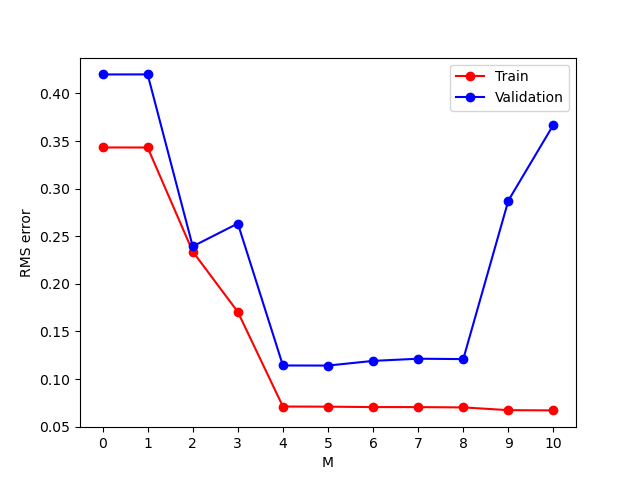
\includegraphics[width=\linewidth]{figures/rms_vs_M.png}
\end{minipage}\hfill
\begin{minipage}{0.38\textwidth}\centering\small
\begin{tabular}{ccc}
\toprule
$M$ & Train & Validation\\\midrule
0 & 0.3433 & 0.4200\\
1 & 0.3432 & 0.4200\\
2 & 0.2339 & 0.2394\\
3 & 0.1705 & 0.2634\\
4 & 0.0711 & 0.1142\\
5 & 0.0710 & \textbf{0.1141}\\
6 & 0.0705 & 0.1191\\
7 & 0.0705 & 0.1213\\
8 & 0.0702 & 0.1209\\
9 & 0.0673 & 0.2875\\
10 & 0.0670 & 0.3671\\\bottomrule
\end{tabular}
\end{minipage}
\end{center}

\paragraph{(c) (3pts)} \textbf{$M=4$} fits best. $M=5$ is only lower by 0.0001, so I'd pick the simpler model. $M\le3$ underfits, since both errors are high. $M\ge9$ overfits: training error keeps going down but validation error jumps up to 0.29 and 0.37.

\paragraph{(d) (3pts)} Done in \texttt{linear\_regression.py}: $\vth=(\Phi^T\Phi+\lambda I)^{-1}\Phi^T\vec y$.

\paragraph{(e) (5pts)} $M=10$. I spaced the $\lambda$ values evenly on the x-axis since 0 can't go on a log scale.
\begin{center}
\begin{minipage}{0.58\textwidth}\centering
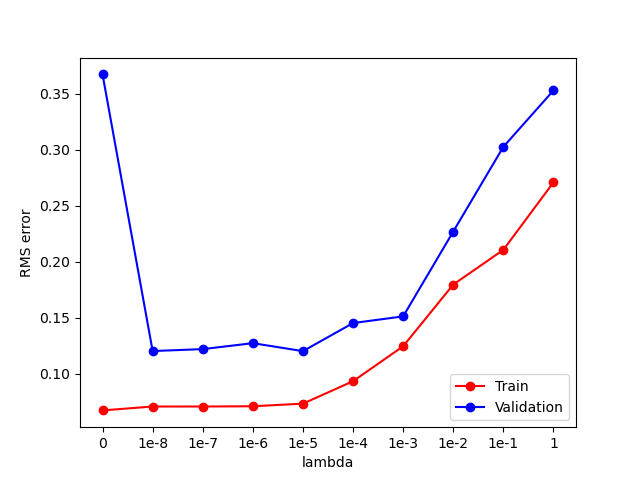
\includegraphics[width=\linewidth]{figures/rms_vs_lambda.png}
\end{minipage}\hfill
\begin{minipage}{0.38\textwidth}\centering\small
\begin{tabular}{ccc}
\toprule
$\lambda$ & Train & Validation\\\midrule
0         & 0.0670 & 0.3671\\
$10^{-8}$ & 0.0705 & 0.1201\\
$10^{-7}$ & 0.0705 & 0.1218\\
$10^{-6}$ & 0.0707 & 0.1271\\
$10^{-5}$ & 0.0731 & \textbf{0.1200}\\
$10^{-4}$ & 0.0931 & 0.1451\\
$10^{-3}$ & 0.1243 & 0.1510\\
$10^{-2}$ & 0.1795 & 0.2268\\
$10^{-1}$ & 0.2104 & 0.3024\\
$10^{0}$  & 0.2707 & 0.3528\\\bottomrule
\end{tabular}
\end{minipage}
\end{center}

\paragraph{(f) (3pts)} \textbf{$\lambda=10^{-5}$} is best (validation 0.1200), though $10^{-8}$ is basically tied. With $\lambda=0$ the model overfits (0.367). Adding even a tiny $\lambda$ cuts validation error to about a third. For $\lambda\ge10^{-4}$ both errors go up, so the model starts underfitting.

\paragraph{(g) (3pts)} I'd pick \textbf{$M=4$ with no regularization}. It has the lowest validation error (0.114 vs.\ 0.120) and it's a simpler model. But with only 20 training and 20 validation points the differences are small and could just be noise, so before deciding I'd use cross-validation over different $(M,\lambda)$ pairs and then check the final model on a separate test set.

\end{document}
